\documentclass{article}
\usepackage[margin=1in]{geometry}
\usepackage{amsfonts}
\usepackage{graphicx}
\usepackage{fancyvrb}
\usepackage{hyperref}

\newcommand{\R}{\mathbb{R}}
\newcommand{\N}{\mathbb{N}}

\title{Some \LaTeX{}  examples}
\author{Geoffrey Matthews}

\begin{document}
\maketitle

\section{Mechanics}
This file contains some examples to get you started using \LaTeX{} to
typeset mathematics.  It is the premiere software for technical
publications.  Good places to get started with tutorials:
\begin{itemize}
\item \url{http://www.latex-tutorial.com/}
\item \url{http://www.stdout.org/~winston/latex/latexsheet.pdf}
\end{itemize}

To compile a \LaTeX{} file, {\tt myfile.tex} to {\tt myfile.pdf}, 
in the labs, simply enter the
following command in a terminal window:
\begin{Verbatim}[frame=single]
pdflatex myfile.tex
\end{Verbatim}
or use a GUI such as TexWorks or TexStudio.

You can also get your \LaTeX\ processed online, for example, at
\begin{itemize}
\item \url{https://www.overleaf.com/}
\item \url{www.sharelatex.com}
\end{itemize}


\section{Some example text}
Here is some inline math:  $\sum_{i=1}^{n} i^2$ and
here is the same thing with display math:
\[
\sum_{i=1}^{n} i^2
\]
Here is a set of equations lined up nicely:
\begin{eqnarray*}
(a+b)^2 &=& (a+b)(a+b) \\
        &=& a(a+b) + b(a+b) \\
        &=& a^2 + ab + ba + b^2 \\
        &=& a^2 + 2ab + b^2
\end{eqnarray*}

You can talk about the real numbers, $\R$, the integers $\mathbb{Z}$, the
rational numbers $\mathbb{Q}$, and the natural numbers,
$\N$, using nice fonts.  Notice how I made new commands for some of these in
the preamble, to simplify typing.
Here is an enumerated list:
\begin{enumerate}

\item $\mathcal{P}(\{1,2,3\}) \subseteq \mathcal{P}(\{1,2,3,4\})$

\item
$
\bigcup_{i\in\N}i^2 = \{0,1,4,9,\ldots\}
$

\item
\[
\bigcap_{i\in\N}i^2 \not= \{0,1,4,9,\ldots\}
\]

\end{enumerate}

\section{Figures}

You can also include and scale figures.
I drew the picture shown in Figure \ref{setfigure}
with a simple paint program, saved it as a {\tt .png}
file, and imported it into this document.


\begin{figure}
  \begin{center}
    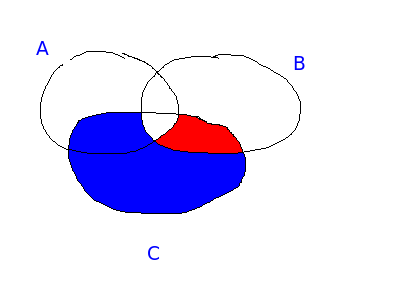
\includegraphics[scale=0.5]{sets.png}
    \caption{A diagram of some sets.}
    \label{setfigure}
  \end{center}
\end{figure}

You can also include figures inline, like this:
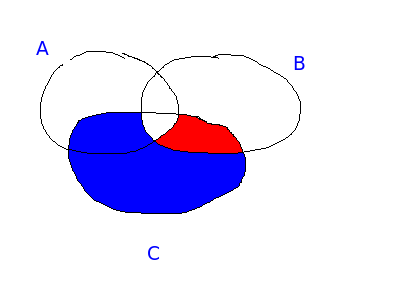
\includegraphics[scale=0.5]{sets.png} but it looks weird sometimes.

Later on, we'll see how to make spectacular diagrams using the {\tt tikz}
package. 

\end{document}
